% !TeX spellcheck = es_ES
% !TeX encoding = UTF-8
% Preambulo{{
\documentclass[10pt,handout]{beamer}
\setbeamersize{text margin left=5mm, text margin right=5mm}
\usetheme{metropolis}

\metroset{numbering=fraction}

% Quitar el fondo de la barra y cambiar el color del texto del título
\setbeamercolor{frametitle}{bg=white, fg=deepblue}

% Opcional: Si quieres que la línea delgada (progress bar) debajo del título 
% también sea azul o desaparezca
\setbeamercolor{progress bar in head/foot}{fg=deepblue, bg=gray!20}
 
% Language{
\usepackage[spanish]{babel}
\usepackage[utf8]{inputenc}
\usepackage[T1]{fontenc}
%}

\usepackage[dvipsnames]{xcolor} 
\usepackage{tikz}
\usetikzlibrary{positioning}

% --- Essentials ---
\usepackage{appendixnumberbeamer}
\usepackage{booktabs}
\usepackage[scale=2]{ccicons}
\usepackage{pgfplots}
\usepgfplotslibrary{dateplot}
\usepackage{xspace}
\usepackage{graphicx}\graphicspath{{figs/}{/home/jadeleon/Documents/doctorado/protocolo_candidatura/gfx/background}{/home/jadeleon/Documents/doctorado/protocolo_candidatura/gfx/chaos_meets_channels/}{/home/jadeleon/Documents/chaos_meets_channels/posters/pix}{../posters/logos/}{../notas/draft/figures/}}
\usepackage{physics}
\usepackage{amsmath}
%\usepackage{siunitx}

% --- Bibliography setup ---
\usepackage[%
    style=verbose,
    backend=bibtex,
    giveninits=true,      % Use initials for first names
    isbn=false, url=false, doi=false, eprint=false,
    maxcitenames=1,
    mincitenames=1
]{biblatex}

% Custom format: Author, Journal, vol, page, (year)
\DeclareFieldFormat[article]{journaltitle}{#1}
\DeclareFieldFormat[article]{volume}{\textbf{#1}} % Bold volume number
\DeclareFieldFormat[article]{pages}{#1} % Remove "p." for cleaner look

% Redefine the short citation format for verbose style
\renewbibmacro*{cite:short}{%
  \color{gray}\tiny
  \printtext[brackets]{%
    \printfield{journaltitle}%
    \setunit*{\space}%
    \printfield{volume}%
    \setunit*{\space}%
    \printfield{pages}%
    \setunit*{\space}%
    \printtext[parens]{\printfield{year}}%
  }
}

% Also modify the full citation format for consistency
\renewbibmacro*{cite:full}{%
  \color{gray}\tiny
  \printtext[brackets]{%
    \printfield{journaltitle}%
    \setunit*{\space}%
    \printfield{volume}%
    \setunit*{\space}%
    \printfield{pages}%
    \setunit*{\space}%
    \printtext[parens]{\printfield{year}}%
  }
}

%\addbibresource{references.bib}
\addbibresource{/home/jadeleon/Documents/doctorado/protocolo_candidatura/references.bib}

% --- Single, clean inline citation command ---
\newcommand{\scite}[1]{\textcolor{gray}{\scriptsize(\citeauthor{#1}, \citeyear{#1})}}

% --- Colors and theme styling ---{
\definecolor{deepblue}{RGB}{46,78,126}
\definecolor{lightblue}{RGB}{200,220,255}
\setbeamercolor{palette primary}{bg=deepblue, fg=white}
\setbeamercolor{palette secondary}{bg=deepblue, fg=white}
\setbeamercolor{palette tertiary}{bg=deepblue, fg=white}
\setbeamercolor{structure}{fg=deepblue}
%}

% --- Title, subtitle, authors, and affiliations ---{
\title{Choi echo: dynamical irreversibility and local decoherence in quantum many-body chaos}
\subtitle{arXiv:2512.11030 \\[5mm]
{\color{gray}\small{9na. Reunión Anual del Grupo de Investigación en caos\\ y termalización en sistemas de muchos cuerpos}}}
\date{}
\author{
\vspace*{-5mm}
\textbf{Jose Alfredo de Leon}\inst{1} \and 
Miguel Gonzalez\inst{2,3} \and
Carlos Diaz-Mejia\inst{2}}
\institute{
\inst{1}Instituto de Física, UNAM
\and 
\inst{2}Instituto de Ciencias Nucleares, UNAM
\and 
\inst{3}\pcs
}
%\titlegraphic{\hfill\includegraphics[height=1cm]{logo.pdf}}
%}

% ------------Other stuff----{
\newcommand{\choip}{\ev{\Tr[\mathcal{D}^2(t)]}_{\mathrm{Haar},t}}
\newcommand{\statep}{\overline{\mathcal{P}}}
\newcommand{\pcs}{Center for Theoretical Physics of Complex Systems, Institute for Basic Science (Corea)}
\newcommand{\mcD}{\mathcal{D}}

\definecolor{azulVibrante}{RGB}{0, 80, 200}
\setbeamercolor{alerted text}{fg=azulVibrante}
\setbeamerfont{alerted text}{series=\bfseries}
%}
%}}
\begin{document}

% ----- Portada -------
\begin{frame} 
\vspace*{-5mm}
\maketitle

% Añade los logos usando TikZ
\begin{tikzpicture}[remember picture, overlay]
  \node[anchor=south east, xshift=-4.15cm, yshift=0.3cm] at (current page.south east){\includegraphics[height=1.2cm]{ifunam.png}};

  \node[anchor=south east, xshift=-1.85cm, yshift=0.3cm] at (current page.south east){\includegraphics[height=1.2cm]{icn.png}};

  \node[anchor=south east, xshift=-0.5cm, yshift=0.3cm] at (current page.south east){
\includegraphics[height=1.25cm]{ibs.png}};

  \node[anchor=center, xshift=-1.8cm, yshift=1.2cm] at (current page.east){\includegraphics[height=2.75cm]{qr_arxiv.pdf}};
\end{tikzpicture}
\end{frame}

\begin{frame}{Colaboradores}

\begin{columns}[T]
\column{0.49\textwidth}
\begin{center}
Miguel Gonzalez\vspace*{5mm}


\includegraphics[width=0.8\columnwidth]{miguel.jpeg}
\end{center}
\vspace*{-2mm}

\column{0.49\textwidth}
\begin{center}
Carlos Diaz-Mejia\vspace*{5mm}

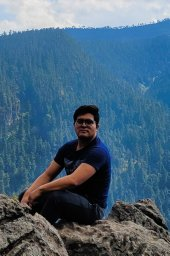
\includegraphics[width=0.6\columnwidth]{charly.jpeg}
\end{center}
\end{columns}
\end{frame}

% ------ Intro, motivación -----
\begin{frame}{Irreversibilidad en sistemas cerrados}
    El \textbf{Echo de Loschmidt} $L(t)$ es la herramienta estándar para caracterizar la sensibilidad a perturbaciones ante una reversión temporal imperfecta:
    \[ L(t) = \abs{\mel{\psi_0}{e^{i(H+\Sigma)t} e^{-iHt}}{\psi_0}}^2 \]
    
    \begin{itemize}
        \item \textbf{Interpretación:} Cuantifica la capacidad de recuperar el estado inicial tras una evolución hacia adelante, una inversión temporal modificada por una perturbación $\Sigma$.
        \begin{center}
        \begin{tikzpicture}[node distance=1.2cm, thick, scale=0.8, transform shape]
            \node (in) {$\ket{\psi_0}$};
            \node (fwd) [right=of in, draw, fill=red!20] {$e^{-iHt}$};
            \node (pert) [right=of fwd, draw, fill=blue!20] {$\Sigma$};
            \node (bwd) [right=of pert, draw, fill=ForestGreen!20] {$e^{iHt}$};
            \node (out) [right=of bwd] {$\ket{\psi_f} \approx \ket{\psi_0}?$};
            
            \draw[->] (in) -- (fwd); \draw[->] (fwd) -- (pert);
            \draw[->] (pert) -- (bwd); \draw[->] (bwd) -- (out);
        \end{tikzpicture}
        \end{center}
        \item \textbf{Física:} Un decaimiento rápido de $L(t)$ es una firma de \alert{irreversibilidad dinámica}.
    \end{itemize}
\cite{goussev_2012_loschmidt,gorin_2006_dynamics}
\end{frame}

\begin{frame}{¿Cómo medir la irreversibilidad en sistemas abiertos?}
    Cuando el sistema $S$ interactúa con un entorno $E$, la dinámica ya no es unitaria, sino que se describe mediante un \textbf{canal cuántico} $\mathcal{E}_t$:
    \[ \rho_S(0) \xrightarrow{\text{Dinámica}} \rho_S(t) = \Tr_E \qty[ U ( \rho_S(0) \otimes \dyad{\psi}_E ) U^\dagger ] \]

    \begin{itemize}
        \item \textbf{El desafío:} El Echo de Loschmidt tradicional depende fuertemente del estado inicial $\ket{\psi_0}$ y de una perturbación Hamiltoniana $\Sigma$.
    \end{itemize}

\metroset{block=fill}
\begin{alertblock}{¿Existe una medida de irreversibilidad que sea intrínseca al canal cuántico $\mathcal{E}_t$? }
Sí, por medio de la pureza de la representación de Choi $\mcD$ de $\mathcal E$ (\alert{echo de Choi}).
\end{alertblock}
\end{frame}

% **** MARCO TEÓRICO *****
% ---- Canales cuánticos ----
\begin{frame}{Canales cuánticos}
\begin{itemize}
\item \textbf{¿Qué describen?} Ruido cuántico, mediciones generalizadas y \alert{dinámica (discreta en el tiempo) de sistemas cuánticos abiertos}. 

\item \textbf{Definición matemática:} $\mathcal E$ es un mapeo completamente positivo que preserva la traza de $\rho$.

\item \textbf{Representaciones de $\mathcal E$:}
\vspace*{-5mm}
\begin{columns}[t,onlytextwidth]
\column{0.49\textwidth}
\metroset{block=fill}
\begin{alertblock}{\color{black}Representación sistema-entorno}
%Para todo $\mathcal{E}$, existe $\{U, \ket{\psi}\}$:
\[
\mathcal{E}(\rho) 
=
\Tr_\mathrm{E}
\qty(
U 
\rho \otimes \dyad{\psi}
U^\dagger
).
\]
%
\begin{center}
\begin{tikzpicture}[font=\large, thick, >=stealth, transform shape, scale=0.8]

% --- Bloque U ---
\draw[rounded corners=6pt, thick] (0,0) rectangle (2,3.5);
\node at (1,2) {$U$};

% --- Bloque E (dentro de U, sombreado) ---
\draw[dashed, rounded corners=6pt, thick] (-0.1,0.1) rectangle (2.1,1.6);
\node at (1,0.85) {$\mathcal{E}$};

% --- Líneas de entrada y salida ---
\draw[-] (-1,0.85) -- (0,0.85);
\draw[-] (-1,2.5) -- (0,2.5);
\draw[-] (2,0.85) -- (3.1,0.85);

% --- Etiquetas de las líneas ---
\node[left] at (-1,2.5) {$\dyad{\psi}$};
\node[left] at (-1,0.85) {$\rho$};
\node[right] at (3.1,0.85)
%    {$\mathrm{Tr}_\mathrm{E}(U \rho \otimes \dyad{\psi} U^{\dagger})$};
     {$\mathcal{E}(\rho)$};
\end{tikzpicture}
\end{center}
\end{alertblock}

\column{0.49\textwidth}
\metroset{block=fill}
\begin{alertblock}{\color{black}Representación de Choi}
A $\mathcal E$ le corresponde un único estado conocido como \alert{estado de Choi}
\[\begin{aligned}
\mathcal{D} &= 
\qty(\mathcal{E} \otimes I )
\qty[\dyad{\Phi}],\\
\ket{\Phi} &= 
\frac{1}{\sqrt{d}}
\sum_i \ket{i}\otimes \ket{i}.
\end{aligned}\]
%\begin{itemize}
%\item 
$\mathcal{D} \in \mathcal{B}(\mathcal H \otimes \mathcal H)$ es una matriz de densidad
%\item $\frac{1}{d^2} \leq \Tr(\mathcal{D}^2) \leq 1$
%\end{itemize}
\end{alertblock}
\end{columns}
\end{itemize}

\end{frame}

\begin{frame}{Ecuación de Lindblad}
    Para una dinámica Markoviana, el mapeo $\mathcal{E}_t$ satisface:
    \[ \mathcal{E}_{t+s} = \mathcal{E}_t \circ \mathcal{E}_s \quad \forall \, t, s \geq 0 \]

    \begin{center}
    \begin{tikzpicture}[node distance=1.5cm, auto, thick, scale=0.9, transform shape]
        % Eje de tiempo
        \draw[->] (-0.5,0) -- (8.5,0) node[right] {$t$};
        
        % Puntos de tiempo
        \foreach \x/\txt in {0/0, 1.5/\Delta t, 3/2\Delta t, 4.5/3\Delta t, 7.5/t} {
            \draw (\x, 0.1) -- (\x, -0.1) node[below] {\footnotesize $\txt$};
        }
        \node at (6, -0.3) {$\dots$};

        % Arcos (Canales)
        \foreach \x in {0, 1.5, 3} {
            \draw[->, bend left=45, azulVibrante] (\x, 0.2) to node[above] {\scriptsize $\mathcal{E}_{\Delta t}$} (\x+1.5, 0.2);
        }
        
        % Canal total
        \draw[->, bend left=35, deepblue] (0, 0.8) to node[above] {$\mathcal{E}_t = \exp(\mathcal{L}t)$} (7.5, 0.8);
        
        % Estado inicial y final
        \node[above] at (0, 0) {$\rho(0)$};
        \node[above] at (7.5, 0) {$\rho(t)$};
    \end{tikzpicture}
    \end{center}

    \begin{itemize}
        \item El canal a tiempo $t$ es la aplicación sucesiva de canales sobre intervalos $\Delta t$:
        \[ \mathcal{E}_t = \underbrace{\mathcal{E}_{\Delta t} \circ \mathcal{E}_{\Delta t} \circ \dots \circ \mathcal{E}_{\Delta t}}_{n = t/\Delta t \text{ veces}} = (\mathcal{E}_{\Delta t})^n \]
        
        \item Al hacer $\Delta t \to 0$, el generador de estos canales es el \textbf{Lindbladiano} $\mathcal{L}$:
        \[ \mathcal{L} = \lim_{\Delta t \to 0} \frac{\mathcal{E}_{\Delta t} - \mathcal{I}}{\Delta t} \implies \mathcal{E}_t = e^{\mathcal{L}t} \]
    \end{itemize}
\end{frame}

% ---- Pureza de Choi ----
%\begin{frame}{Pureza de Choi $\Tr(\mathcal{D}^2)$}
%\begin{itemize}
%\item $\Tr(\mathcal{D}^2)$ cuantifica la no unitariedad del canal $\mathcal E$,
%\[
%\text{ (máximo ruido) } \frac{1}{d_S^2} \leq \Tr(\mathcal{D}^2) \leq 1 \text{ (unitario)}.
%\]
%
%\item Proporciona más información que la pureza de estados finales:
%\[
%\mathbb{E} \left[ \Tr(\mathcal{E}(\dyad{\psi})^2) \right] = \frac{1}{d_S(d_S + 1)} \bigg(  \Tr[\mathcal{E}(\mathbb{I}_S)^2] 
%+ d_S^2 \Tr(\mathcal{D}^2) \bigg),
%\]
%donde $\mathbb{E}[\cdot]$ denota el promedio de Haar al muestrar estados puros 
%$\ket{\psi}$ del sistema. 
%
%\item Para un canal unitario y un canal que mapea todos los estados al estado $\ket{0}$ $\Tr(\mathcal{E}(\dyad{\psi})^2) = 1$, mientras que $\Tr(\mathcal{D}^2)=1, 1/2$, respectivamente.
%\end{itemize}
%\end{frame}

\begin{frame}{Pureza de Choi $\Tr(\mathcal{D}^2)$}
\begin{itemize}
  \item \textbf{Medida de unitariedad:} Cuantifica la no-unitariedad de $\mathcal E$.
  \[ \frac{1}{d_S^2} \text{ (ruido máx.)} \leq \Tr(\mathcal{D}^2) \leq 1 \text{ (unitario)} \]
  \begin{quote}
    \small \textit{Ejemplo:} Evolución unitaria ($\Tr(\mathcal{D}^2)=1$) vs. Canal de amortiguamiento de amplitud, $\mathcal{E}(\rho) = \dyad{0}$ ($\Tr(\mathcal{D}^2)=1/d_S$). \alert{La pureza de estados no puede distinguir estos dos procesos distintos.}
  \end{quote}

  \item \textbf{Relación con la pureza promedio:} Determina la pureza de los estados finales promediada sobre la medida de Haar:
  \[
  \mathbb{E} \left[ \Tr(\mathcal{E}(\dyad{\psi})^2) \right] = \frac{1}{d_S(d_S + 1)} \bigg( \Tr[\mathcal{E}(\mathbb{I}_S)^2] + d_S^2 \Tr(\mathcal{D}^2) \bigg)
  \]
  
\end{itemize}
\end{frame}


% --- Echo de Choi ----
\begin{frame}{Echo de Choi: interpretación operacional de $\Tr(\mathcal{D}^2)$}
Para un canal cuántico arbitrario 
$\mathcal{E}(\rho) = \Tr_\mathrm{E} \qty( U \rho \otimes \dyad{\psi} U^\dagger)$:
\[
  \Tr(\mathcal{D}^2) = 
  \ev**{
  \Tr_{S}\qty{
  {\color<4->{ForestGreen} U^\dagger} 
  {\color<3->{blue}\Lambda \qty[
  {\color<2->{red} U} 
  {\color{black} \left( \frac{\mathbb{I}_{S}}{d_{S}} \otimes \dyad{\psi} \right)} 
  {\color<2->{red} U^\dagger}
  ]}
  {\color<4->{ForestGreen} U}
  }
  }{\psi},
\]
donde $\Lambda(\cdot) = \mathbb{I}_S/d_S\Tr_S\pqty{\cdot}$.

Es decir, $\Tr(\mathcal{D}^2)$ es la probabilidad de recuperar al entorno en 
$\ket{\psi}$ después de:
\begin{enumerate}
  \item<2-> Evolución para adelante con {\color<2->{red} $U$} 
  \item<3-> Un proceso local (sobre $S$) de máximo ruido {\color<3->{blue} $\Lambda$} \alert{que borra el entrelazamiento entre $S$ y $E$.}
  \item<4-> Evolución para atrás con {\color<4->{ForestGreen} $U^\dagger$}
\end{enumerate}

\uncover<5->{
    \textbf{La pureza de Choi cuantifica la irreversibilidad de la evolución
    ante una perturbación que destruye el entrelazamiento, por eso, \alert{\textit{echo de Choi}.}}
}

%\begin{tikzpicture}[overlay, remember picture, shift={(current page.center)}]
%\visible<5->{
%    \node[fill=orange!30, 
%          draw=orange!80!black,
%          thick,
%          rounded corners=10pt,
%          inner sep=5pt,
%          minimum width=0.35\linewidth,
%          align=center] at (4, -1.5) {
%        \textcolor{orange!80!black}{Echo de Loschmidt}\\
%        \textcolor{black}{$\mel{\psi_0}{e^{i (H + V) t}e^{-i H t}}{\psi_0}$}
%    };
%}
%\end{tikzpicture}
\end{frame}

\begin{frame}{Decoherencia de un subsistema como indicador de caos}
%\begin{itemize}
%  \item Propiedades estadísticas del Hamiltoniano $\rightarrow$ matriz aleatoria
%
%  \item Desafío: Acceso limitado a propiedades completas del sistema
  \begin{columns}[T]
  \column{0.49\textwidth}
  
  Señales espectrales de caos: \alert{difícil}
    \begin{center}
      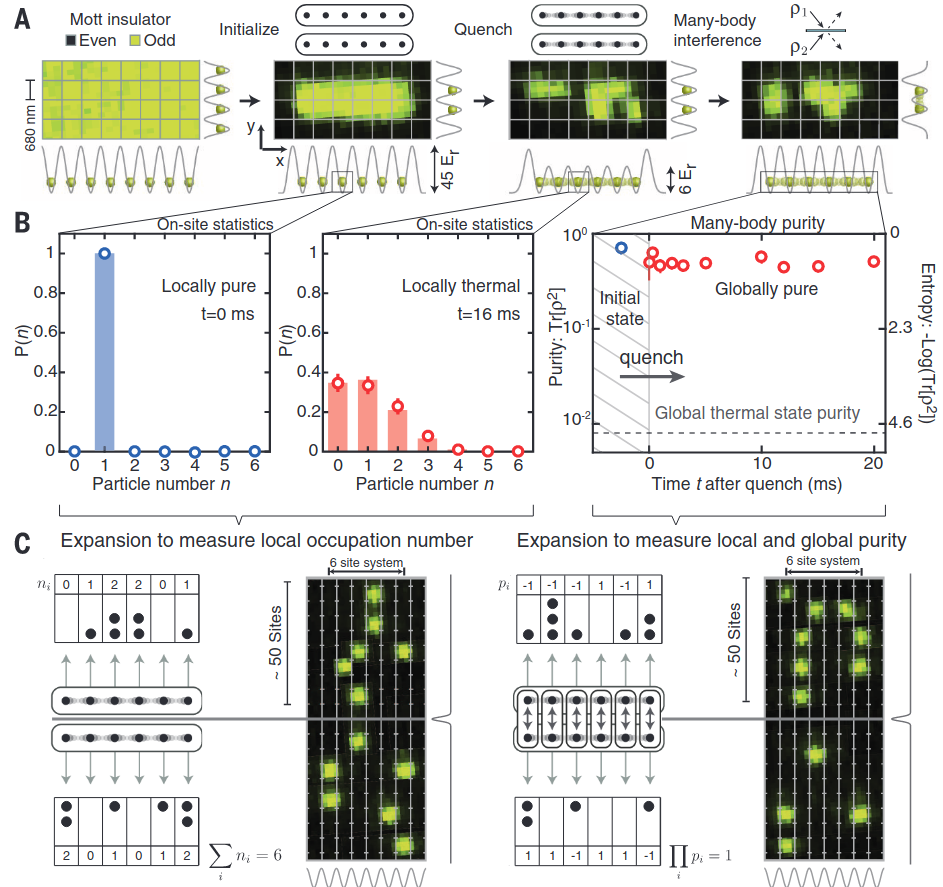
\includegraphics[width=0.8\textwidth]{bose_hubbard_greiner.png}
    \end{center}
    \vspace*{-5mm}\hfill \cite{kaufman_2016_quantum}

    \begin{columns}[c] % [c] asegura el centrado vertical
    \column{0.56\textwidth}
        \centering
        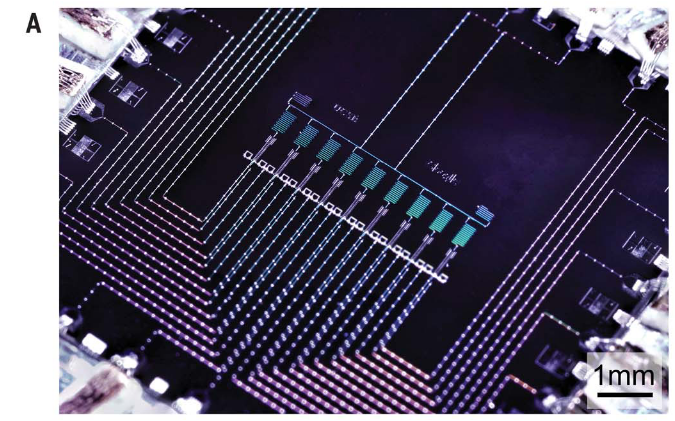
\includegraphics[width=\linewidth]{superconducting_chip.png}
        
    \column{0.43\textwidth}
        \centering
        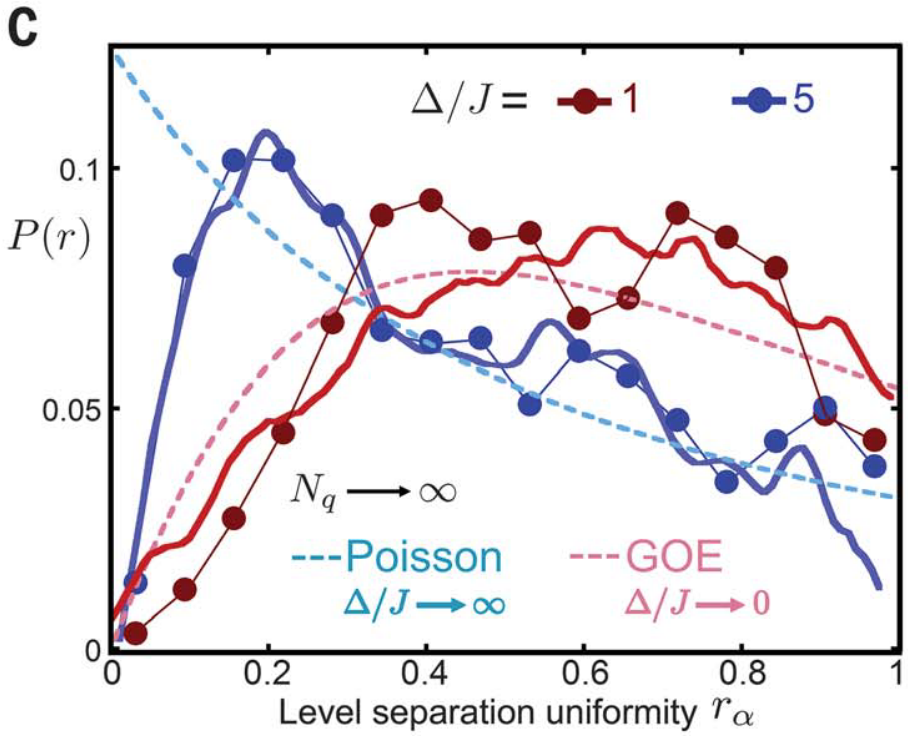
\includegraphics[width=\linewidth]{ratios_distribution_chip.png}
    \end{columns}
    \hfill \cite{roushan_2017_spectroscopic}
  
  \column{0.49\textwidth}
    Señales de caos en subsistemas
    \begin{center}
    \includegraphics[width=0.85\linewidth]{fig1_mirkin.png}
    \end{center}
    \vspace*{-5mm}\hfill \cite{mirkin_2021_quantum}

    \begin{center}
    \includegraphics[width=0.85\linewidth]{fig1_mirkin2021b.png}
    \end{center}
    \vspace*{-5mm}\hfill \cite{mirkin_2021_sensing}
  \end{columns}
%\end{itemize}
\end{frame}

%\begin{frame}{Caos cuántico monitoreando sistemas reducidos}
%\end{frame}

%\begin{frame} % Opening, motivation
%\vspace*{-5mm}
%\begin{center}
%\includegraphics[height=\textheight]{idea.pdf}
%\end{center}
%
%%\begin{center}
%\begin{tikzpicture}[overlay, remember picture, shift={(current page.center)}]
%% Caja con fondo degradado
%\node[fill=orange!30, 
%      draw=orange!80!black,
%      thick,
%      rounded corners=10pt,
%      inner sep=5pt,
%      minimum width=0.6\linewidth,
%      align=center] at (0,-3.8) {
%    \textcolor{orange!80!black}{¿Señales de caos en el canal cuántico $\mathcal{E}$?}\\
%    \textcolor{black}{\textbf{Pureza de Choi}}
%};
%
%\end{tikzpicture}
%%\end{center}
%\end{frame}

% --- Quantum chaos ----
\begin{frame}[t]{Caos cuántico}
\begin{columns}[onlytextwidth]
\column{0.35\textwidth}

\metroset{block=fill}
\begin{alertblock}{\color{black} Caos cuántico = RMT}
\begin{center}
\includegraphics[width=0.95\textwidth]{random_goe.pdf}
\end{center}
\end{alertblock}

\column{0.63\textwidth}
\vspace*{-2mm}
\metroset{block=fill}
\begin{alertblock}{Eigenvalores correlacionados}
\begin{itemize}
\item Repulsión de niveles
\hspace*{27mm}
\includegraphics[height=25mm,page=2]{spacings.pdf}
\vspace*{-3mm}
\item $SFF(t) = \sum_{i,j} e^{-i (E_i - E_j) t}$
\begin{center}
\includegraphics[height=24mm]{sff.png}
\end{center}
\end{itemize}
\vspace*{-2mm}
\end{alertblock}

\begin{exampleblock}{Eigenvectores deslocalizados}
\vspace*{-2mm}
\begin{center}
$\ket{E_i} \approx \ket{\psi_{\mathrm{random}}}$
\end{center}
\vspace*{-2mm}
\end{exampleblock}
\end{columns}

%\vspace*{-5mm}
%\cite{bohigas_1984_characterization}
%\cite{berry_1997_level}

\begin{tikzpicture}[overlay, remember picture, shift={(current page.center)}]
\node[xshift=4mm, yshift=20mm] at (current page.center) 
{\tiny$
\begin{aligned}
\tilde r_n &= \frac{E_{n+1} - E_n}{E_{n} - E_{n-1}},
r_n = \min\left(\tilde r_n, \frac{1}{\tilde r_n}\right)
%r_n = \min\qty( \frac{E_{n+1} - E_n}{E_{n} - E_{n-1}}, \frac{E_{n+1} - E_n}{E_{n} - E_{n-1}})
\end{aligned}
$};
%
\node[xshift=2mm, yshift=12mm] at (current page.center) 
{\tiny $
\begin{aligned}
\ev{r}_{\mathrm{GOE}} &\approx 0.536 \\
\ev{r}_{\mathrm{Poisson}} &\approx 0.386
\end{aligned}
$};
%
\node[xshift=7mm, yshift=4mm] at (current page.center) 
{\tiny \color{gray} [PRL \textbf{110} 084101 (2013)]};
\end{tikzpicture}
\end{frame}

\begin{frame}{Pureza de Choi como indicador de caos}
Dado un Hamiltoniano $H$,
\begin{equation*}
\mathcal{E}_t(\rho) 
=
\Tr_\mathrm{E}
\qty(
e^{-i H t}
\rho \otimes \dyad{\psi}
e^{i H t}
),\quad 
\ket{\psi} = \bigotimes_i \ket{\phi_i}.
\end{equation*}

\begin{columns}[T,onlytextwidth]
\column{0.49\textwidth}
\textbf{¿Cómo se ve el canal cuántico $\mathcal E_t$?}

\vspace*{2mm}

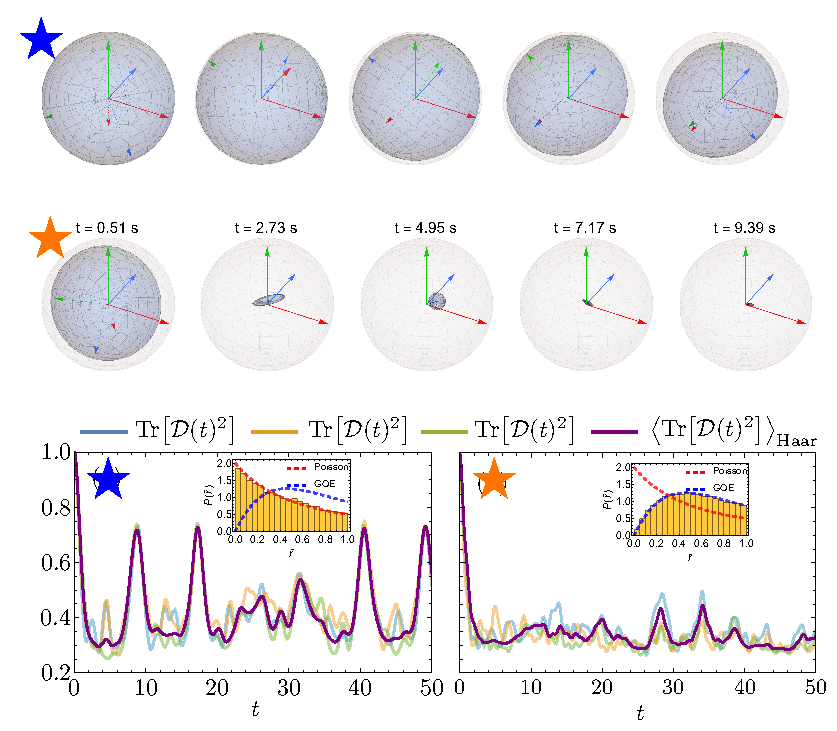
\includegraphics[width=\linewidth]{channel.pdf}

\column{0.49\textwidth}
\metroset{block=fill}
\begin{alertblock}{Promedio de Haar de $\Tr[\mathcal{D}(t)^2]$}
\begin{itemize}
\item El caos está en $H$
\item Sin embargo, $\mathcal E$ depende de $\ket{\psi}$
\item Removemos \alert{analíticamente} la dependencia en $\ket{\psi}$: 
\vspace*{-4mm}
\begin{equation*}
\scalebox{0.45}{$
\underset{\ket{\phi_i} \sim \mu_{\mathrm{Haar}} }
{\mathbb{E}\qty[\Tr \mathcal{D}^2(t)]} 
= 
\frac{1}{12^{L-1}} \sum_{\vec{k} \in 
\{0,1,2,3\}^{L-1}} 3^{\frac{1}{2}\qty(L - 1 - w\qty(\vec{k}))} 
\Tr \qty[ \Tr_S^2 \qty(U(t) \sigma_{0,\vec{k}}\, U^\dagger(t)) ]
$}
\end{equation*}

\item \alert{Vamos a usar el siguiente número como indicador de caos:}
\begin{equation*}
\scalebox{0.9}{$
\ev{\Tr \mathcal{D}^2(t)}_{\mathrm{Haar}, t} = 
\int_0^T
\underset{\ket{\phi_i} \sim \mu_{\mathrm{Haar}} }
{\mathbb{E}\qty[\Tr \mathcal{D}^2(t)]} 
\dd{t}
$}
\end{equation*}
\end{itemize}
\end{alertblock}
\end{columns}

\end{frame}

% --- Resultados ---
\begin{frame}{Modelo de Ising con campos transverso y longitudinal}
\[
H = \sum_{i=1}^L \left( h_x \sigma_i^x + h_z \sigma_i^z \right) 
- J \sum_{i=1}^{L-1} \sigma_i^z \sigma_{i+1}^z,
\]
\vspace*{-12mm}
\begin{center}
\begin{tikzpicture}
\begin{scope}[shift={(0,0)}]
% Mean level spacing ratio{{{
\node (listdensityplotr) at (0,0) 
  {
\includegraphics[width=0.325\textwidth]{mean_level_spacing_ratio_ising_L_16_hx_1_even_parity.pdf}};% mapa de color
\node (barlegend) at (listdensityplotr.north) [anchor=south, inner sep=-10pt]  {
\includegraphics[width=0.27\textwidth]{mean_level_spacing_ratio_ising_bar_legend.pdf}};% barra de leyenda

%Etiquetas 
\node[rotate=90] () at (listdensityplotr.west) [] {$J/h_x$};
\node (labelr) at (barlegend.north) [anchor=south, inner sep=8pt] {$\ev{\tilde r}$};
\node () at (listdensityplotr.south) [anchor=north, inner sep=-5pt] {$h_z/h_x$};
%}}}

% Averaged purity{{{
\node (chaometer) at ([xshift=-10pt,yshift=-0.2pt]listdensityplotr.east) [anchor=west] 
  {
\includegraphics[height=0.345\textwidth]{chaometer_purity_ising_L_7_hx_1.pdf}};%mapa de color
\node (legendChaometer) at (chaometer.north) [anchor=south, inner sep=-10pt]  
  {
\includegraphics[width=0.27\textwidth]{chaometer_purity_ising_bar_legend.pdf}};% bara para leyenda

\node (labelChaometer) at (legendChaometer.north) [anchor=south, inner sep=9pt] {$\overline{\mathcal{P}}$};
\node () at (chaometer.south) [anchor=north, inner sep=-5pt] {$h_z/h_x$};
%}}}

% Averaged Choi purity{{{
\node (choi) at ([xshift=-6.5pt,yshift=-2pt]chaometer.east) [anchor=west] 
  {
\includegraphics[height=0.33\textwidth]{temporal_avg_haar_avg_choi_purity_ising_L_7_hx_1.pdf}};% mapa de color
\node (legendChoi) at (choi.north) [anchor=south, inner sep=-2pt]  
  {
\includegraphics[width=0.27\textwidth]{temporal_avg_haar_avg_choi_purity_ising_bar_legend.pdf}};% barra de leyenda
%
\node (labelchoi) at (legendChoi.north) [anchor=south, inner sep=2pt] {$\ev{\Tr[\mcD(t)^2]}_{\mathrm{Haar}, t}$};
\node () at (choi.south) [anchor=north, inner sep=-5pt] {$h_z/h_x$};
%}}}

% Letras{{{
\node (a) at ([xshift=-1.56cm, yshift=0.1cm]labelr.west) {(a)};
\node (b) at ([xshift=3.8cm, yshift=0pt]a.east) {(b)};
\node (c) at ([xshift=3.5cm, yshift=0pt]b.east) {(c)};
%}}}

\draw[red, dashed, line width=0.9pt, opacity=0.7] (-1.76,-0.5) -- (1.85,-0.5);
\draw[red, dashed, line width=0.9pt, opacity=0.7] (2.05,-0.5) -- (5.65,-0.5);
\draw[red, dashed, line width=0.9pt, opacity=0.7] (5.85,-0.49) -- (9.45,-0.49);

\end{scope}
\end{tikzpicture}
\end{center}

\begin{itemize}
\item Arriba de la línea roja punteada la decoherencia funciona como indicador 
\item Abajo de la línea roja punteada la decoherencia no funciona como indicador
\end{itemize}
\end{frame}

\begin{frame}{Modelo de Heisenberg con campos aleatorios}

\[
H = \frac{1}{4}\sum_{i=1}^{L-1} \left(\sigma_i^x\sigma_{i+1}^x 
+ \sigma_i^y\sigma_{i+1}^y + \sigma_i^z\sigma_{i+1}^z\right) 
+ \frac{1}{2}\sum_{i=1}^L h_i \sigma_i^z,
\quad 
h_i \sim [-h,h]
\]
\begin{center}
\begin{tikzpicture}
\begin{scope}[anchor=north west, shift={(0,-8.9)}, scale=0.95, transform shape]
\node[anchor=north west] (g) at (0, 0) {
\includegraphics[width=0.65\textwidth]{heisenberg.pdf}};
\node () at (g.south) [anchor=north, inner sep=-5pt] {$h$};
\node(label1) at (1.4,-3) {$7$ $\uparrow$};
\node(label2) at ([xshift=0pt,yshift=-5pt]label1.north) [anchor=south] {$13$ $\uparrow$};
\node(label3) at ([xshift=0pt,yshift=-3pt]label2.north) [anchor=south, inner ysep=0pt] {$6$ $\uparrow$};
\node(label4) at ([xshift=0pt,yshift=1pt]label3.north) [anchor=south, inner ysep=0pt] {$5$ $\uparrow$};
\node(label5) at ([xshift=0pt,yshift=2pt]label4.north) [anchor=south, inner ysep=0pt] {$4$ $\uparrow$};
\node() at ([xshift=-7pt,yshift=3pt]label5.north) [anchor=south, inner ysep=0pt] {$\ev{\tilde r}$};

\node(labelgoe) at (4.2, -0.43) {$\ev{\tilde{r}}_\mathrm{GOE}$};
\node() at ([xshift=7pt,yshift=0pt]labelgoe.east) [anchor=west, inner sep=0pt] {$\ev{\tilde{r}}_\mathrm{Poisson}$};
\node(labelChoi) at ([xshift=-18pt,yshift=4pt]labelgoe.south) [anchor=north west] {\small $1 - \ev{\Tr[\mathcal{D}(t)^2]}_{\mathrm{Haar},t}$};
\node(labelP) at ([xshift=-30pt,yshift=8pt]labelChoi.south) [anchor=north] {\small $1- \overline{\mathcal{P}}$};
\end{scope}
\end{tikzpicture}
\end{center}

\begin{itemize}
\item $\choip$ tiene una desviación estándar no visible al ojo
en la región de caos
\end{itemize}
\end{frame}

\begin{frame}{Modelo XXZ con defecto local}
\[
H = \frac{1}{4}\sum_{i=1}^{L-1} \left[ J_{xy} \left(\sigma_i^x\sigma_{i+1}^x 
+ \sigma_i^y\sigma_{i+1}^y \right) + J_z \sigma_i^z\sigma_{i+1}^z \right] 
+ \frac{1}{2}\varepsilon \sigma_d^z.
\]
\vspace*{-10mm}
\begin{center}
\begin{tikzpicture}
\begin{scope}[shift={(0,-6)}]
% Mean level spacing ratio{
\node (listdensityplotr) at (0,0.05) {
\includegraphics[width=0.325\textwidth]{../notas/draft/figures/mean_level_spacing_ratio_xxz_L_18_spinsUp_7_d_9_omega_0.pdf}};
\node[rotate=90] () at ([xshift=-3pt,yshift=0pt]listdensityplotr.west) [] {$J_{xy}/J_z$};
\node (barlegend) at (listdensityplotr.north) [anchor=south, inner sep=-7pt]  {
\includegraphics[width=0.27\textwidth]{mean_level_spacing_ratio_ising_bar_legend.pdf}};
\node (labelr) at (barlegend.north) [anchor=south, inner sep=8pt] {$\ev{\tilde r}$};
\node () at (listdensityplotr.south) [anchor=north, inner sep=-5pt] {$\varepsilon/J_z$};
%}

% Averaged purity{
\node (chaometer) at ([xshift=-7pt,yshift=-2.3pt]listdensityplotr.east) [anchor=west] {
\includegraphics[height=0.333\textwidth]{chaometer_purity_xxz_open_L_7_d_3_Jz_1.00_omega_0.00.pdf}};
\node (legendChaometer) at (chaometer.north) [anchor=south, inner sep=-2pt]  {
\includegraphics[width=0.27\textwidth]{chaometer_purity_xxz_bar_legend.pdf}};
\node (labelChaometer) at (legendChaometer.north) [anchor=south, inner sep=5pt] {$\overline{\mathcal{P}}$};
\node () at (chaometer.south) [anchor=north, inner sep=-5pt]
 {$\varepsilon/J_z$};
%}

% Averaged Choi purity{
\node (choi) at ([xshift=-6.5pt,yshift=0pt]chaometer.east) [anchor=west] {
\includegraphics[height=0.333\textwidth]{temporal_avg_haar_avg_choi_purity_xxz_L_7_Jz_1_omega_0_d_3.pdf}};
\node (legendChoi) at (choi.north) [anchor=south, inner sep=-2pt]  {
\includegraphics[width=0.27\textwidth]{temporal_avg_haar_avg_choi_purity_xxz_bar_legend.pdf}};
\node (labelchoi) at (legendChoi.north) [anchor=south, inner sep=2pt] {$\ev{\Tr[\mcD(t)^2]}_{\mathrm{Haar}, t}$};
\node () at (choi.south) [anchor=north, inner sep=-5pt] {$\varepsilon/J_z$};
%}

% Letters{
\node (a) at ([xshift=-1.65cm, yshift=0.1cm]labelr.west) {(a)};
\node (b) at ([xshift=3.85cm, yshift=0pt]a.east) {(b)};
\node (c) at ([xshift=3.5cm, yshift=0pt]b.east) {(c)};
%}
\end{scope}
\end{tikzpicture}
\end{center}

\begin{itemize}
\item Detección espuria de caos.
\end{itemize}
\end{frame}

% --- Thank you slide ---
\begin{frame}[standout]
  \centering
  Muchas gracias, ¿preguntas?\\
  \vspace{1cm}

  \includegraphics[height=4cm]{qr_arxiv.pdf}

  arXiv:2512.11030\\
  \vspace{1cm}
  \small Jose Alfredo de Leon\\
  \texttt{deleongarrido.jose@gmail.com}\\
%  \vspace{0.5cm}
%  \tiny References available upon request
\end{frame}

% --- References slide ---
%\begin{frame}[allowframebreaks]{References}
%  \printbibliography[heading=none]
%\end{frame}

\end{document}